\chapter{Apprentissage Machine d'Architectures Profondes}


\section{Introduction à l'Apprentissage Statistique}

L'apprentissage machine est un champ de recherche de l'intelligence
artificielle. Il permet notamment d'extraire des informations utiles à l'aide à
la décision.  L'objectif ici est de pouvoir extraire de manière quasiment
automatique à partir de grandes masses de données une information pertinente.
C'est l'immense quantité de données (ou leur dimensionnalité trop élevée)  qui
rend cette tâche difficile, parfois impossible, à accomplir pour un être
humain.


\subsection{Formalisation du Problème}

L'objectif est de trouver une fonction $f\in\mathcal{F}$ qui va exécuter une
tâche particulière. Il faut donc définir l'espace des fonctions $\mathcal{F}$
parmi lequel nous allons chercher la solution optimale à notre problème.  Il
faut également définir une fonction de coût ou d'objectif $\mathcal{C}$ qui
évalue retourne un réél $\mathcal{C}(\mathcal{D},f)\in\mathbb{R}$ nous
permettant d'évaluer la qualité d'une fonction donnée sur un échantillon de
données $\mathcal{D}$.

La solution à notre problème est donc la fonction $f^*$ définie par:

\begin{equation}
\label{eq:graal}
f^* = \argmin_{f \in \mathcal{F}} {\mathbb E}_\mathcal{D}[\mathcal{C}(\mathcal{D},f)]
\end{equation}


En supposant qu'on ait accès à une infinité de données, nous serions en mesure
de calculer de façon exacte le {\bf risque espéré} ${\mathbb
E}_\mathcal{D}[\mathcal{C}(\mathcal{D},f)]$. Malheureusement, l'ensemble de
données $\mathcal{D}$ est de taille finie et on ne peut disposer que d'un estimé
du risque espéré. L'idée est de minimiser l'objectif sur un ensemble d'entraînement
$\mathcal{C}(\mathcal{D}_\textrm{train},f)$ puis d'approximer le risque espéré sur un ensemble
qui n'a pas été vu lors de l'apprentissage, un ensemble de test
$\mathcal{D}_\textrm{test}$. On va donc minimiser le {\bf risque empirique} sur
l'ensemble d'entraînement:

\begin{equation}
\label{eq:graal}
\hat{f}^* = \argmin_{f \in \mathcal{F}} \mathcal{C}(\mathcal{D}_\textrm{train},f)]
\end{equation}

Pour une quantité de données limitée, il est possible de trouver une fonction
$f\in\mathcal{F}$ qui donne un risque empirique proche de $0$ pourvu que
$\mathcal{F}$ définisse un espace de fonctions à la complexité assez élevée (il
est parfois possible de mesurer cette complexité avec la dimension de
Vapnik-Chervonenkis~\cite{Vapnik71}). Mais ceci ne résulte pas nécessairement en une solution
qui généralise bien sur de nouvelles données qui n'ont pas été utilisées au
cours de l'entraînement. Ceci est un phénoméne appelé \emph{sur-apprentissage}:
on a un risque empirique faible sur l'ensemble d'entraînement et un risque
espéré élevé. 

Afin de réduire l'écart de performance en généralisation entre la solution du
problème de minimisation du risque empirique $\hat{f}^*$ et la solution de
l'Eq.~\ref{eq:graal} dénotée $f^*$, une des alternatives consiste à réduire
l'espace $\mathcal{F}$ des fonctions à des fonctions d'une complexité moins
élevée. On peut aussi ajouter une pénalité de régularisation sur la complexité
de la fonction $f$ contrôlée par un coefficient $\lambda$. Une régularisation
trop forte peut parfois aboutir à du \emph{sous-apprentissage}.  \\

En général, un ensemble de données est découpé en $3$ ensembles disjoints.


\begin{itemize}

\item L'{\bf ensemble d'apprentissage} $\mathcal{D}_\textrm{train}$ pour la
minimisation du risque empirique et l'entraînement des paramètres de la
fonction $f$.

\item L' {\bf ensemble de validation} $\mathcal{D_{\mathrm{valid}}}$ permet de
choisir les hyper-paramtètres de l'algorithme d'apprentissage comme par exemple
la pénalité de régularisation $\lambda$.

\item L'{\bf ensemble de test} $\mathcal{D_{\mathrm{test}}}$  permet d'avoir un
approximé du risque espéré.

\end{itemize}


\subsection{Réseaux de Neurones Artificiels}

On restreint ici l'espace des fonctions $\mathcal{F}$ à celui des réseaux de
neurones à plusieurs couches plus communément appelés Perceptron Multi-Couches,
en anglais \textit{Multi-Layer Perceptron} (MLP)\cite{Rosenblatt-1958}. Soit
$x\in\mathbb{R}^d$ l'entrée fournie au réseau. On fixe $x=h^{(0)}$. La sortie
$h^{(i)}(x)$ d'une couche $i$ est définie comme la projection affine
$W^{(i)}h^{(i-1)}(x) + b^{(i)}$ des données de la couche inférieure $h^{(i-1)}(x)$
suivie d'une non-linéarité $h^{(i)}(x)= s(W^{(i)}h^{(i-1)}(x) + b^{(i)})$, en
général la fonction logistique $s(x)=1/(1+e^{-x})$ qui est différentiable et
permet l'application de l'algorithme de rétro-propagation du gradient. 

La dernière couche d'un réseau de neurones pour résoudre un problème de
classification a en général la forme d'une régression logistique multinomiale
avec autant d'unités que de classes. La sortie d'un réseau à $m$ couches pour
$K$ classes est donnée par

\begin{equation}
o(x) = \frac{e^{W^{(m+1)} h^{(m)}(x) + b^{m+1}}}{\sum_{j=1}^K e^{W^{(m+1)}_{k.} h^{(m)}(x) + b^{(m+1)}_k }}
\end{equation}

où $W_{k.}^{(m+1)}$ désigne la $k^\textrm{ième}$ ligne de la matrice $W^{(m+1)}$
et $b_k^{(m+1)}$ la $k^\textrm{ième}$ composante du vecteur $b^{(m+1)}$.
\\

Les MLPs s'entraînent par rétropropagation du gradient \cite{Rumelhart86b}: c'est une application
astucieuse de la régle de dérivée en chaîne et de la programmation dynamique
pour que cela soit effectué de manière efficiente.
\\

Depuis \cite{Hinton06,Bengio-nips-2006}, il a été démontré qu'il peut être
avantageux de pré-entraîner un réseau de neurones en utilisant des algorithmes
d'extraction de caractéristiques en apprentissage non supervisé. Plutôt que
d'initialiser les paramètres de chaque couche $\lbrace W,b \rbrace$ de façon
aléatoire, on les initialise avec les paramètres résultant de l'apprentissage
non supervisé.  Cela permet d'obtenir de nettes améliorations de performances
et d'entraîner des réseaux à plusieurs couches de manière efficace.

Dans ce qui suit, nous présenterons les techniques d'apprentissage non
supervisé les plus couramment utilisées pour l'extraction de caractéristiques
et le pré-entraînement de réseaux de neurones.


\section{Historique et Méthodologie}

Dans cette partie, nous chercherons à décrire les avancées historiques qui ont
permis d'aboutir au modèle du perceptron multi-couches. C'est cette
architecture qui nous servira de base pour la suite de ce mémoire. Commençons
avec un bref descriptif d'un réseau de neurones naturel que nous possédons
tous: le cerveau.

\subsection{Réseaux de Neurones Naturels}

\subsubsection{Le cerveau humain}

Le cerveau humain est composé de milliers de neurones ($\simeq 10^{11}$)
connectés entre eux en un immense réseau. Nous sommes encore très loin de tout
savoir sur son fonctionnement... À première vue, on peut le considérer comme
une "boîte noire" qui traite en continu une large variété d'entrées et retourne
des "instructions" aux muscles, le tout avec un haut degré de parallélisme.
C'est ce qui nous permet par exemple de respirer et réfléchir au même moment.

On peut supposer que le cerveau fonctionne ainsi: à chaque stimulus présenté en
entrée, l'ensemble des neurones s'adapte par une suite d'activations et
d'inhibitions dans un laps de temps très court pour former un patron
d'activation. Ce patron d'activation est composé de: \\

\begin{itemize}
\item neurones actifs, soit environ $1\%$ de tous les neurones:
\begin{enumerate}
\item les neurones \underline{excitateurs} qui vont libérer une charge électrique qui excite les neurones de leur voisinage.
\item les neurones \underline{inhibiteurs} qui vont libérer une charge électrique qui inhibe les neurones de leur voisinage.
\end{enumerate}
\item et de neurones passifs ne réagissant pas à ce type d'entrée \textit{id est} leur activation est nulle.
\\
\end{itemize}

Formellement, pour un système contenant $d$ unités cachées (neurones), un
patron d'activation est un vecteur à $d$ dimensions représentant les valeurs
d'activation de chaque unité. 

La supposition précédente, déjà bien ancrée dans la communauté scientifique,
est le principe de base du \textbf{connectionnisme}. On suppose que le
fonctionnement d'un système "intelligent" et complexe comme notre cerveau peut
être décrit à l'aide de réseaux d'unités simples (neurones connectés entre eux
par des synapses).

En ce qui nous concerne, on espère qu'un tel système soit capable
d'apprentissage, c'est à dire qu'il soit à terme capable d'associer tel patron
d'activation à tel stimulus présenté en entrée. Le processus d'apprentissage
passe par l'ajustement des connections (poids) entre les différentes unités. En
effet, une fois la configuration d'un réseau fixée, les poids sont les seuls
paramètres qu'il nous est possible de modifier. La \textbf{connaissance} d'un
tel réseau réside donc dans la valeur des connections entre ses unités.

\subsubsection{Neurone biologique}

Chacun des noeuds de ce réseau naturel qu'est le cerveau correspond à un
neurone. Sans entrer dans les détails, le neurone est grossièrement composé de
trois éléments: les dendrites, le corps cellulaire et l'axone. Les
\textbf{dendrites} forment un ensemble de récepteurs nerveux répartis au
voisinage du corps celllulaire. Ces récepteurs captent le potentiel électrique
en provenance d'autres neurones. Si les dendrites accumulent une charge
dépassant un certain seuil, le \textbf{corps cellulaire} émet un potentiel
électrique (via son \textbf{axone}) susceptible d'exciter ou d'inhiber les
neurones aux alentours, plus précisément ceux dont les dendrites sont
connectées à l'axone par des synapses (d'où le nom de \textbf{connections
synaptiques}). On dénombre environ $10^{4}$ connections par neurone. Une vue
schématique d'un neurone est présentée en figure  \ref{fig:neurobio}.

\begin{figure}
\begin{center}
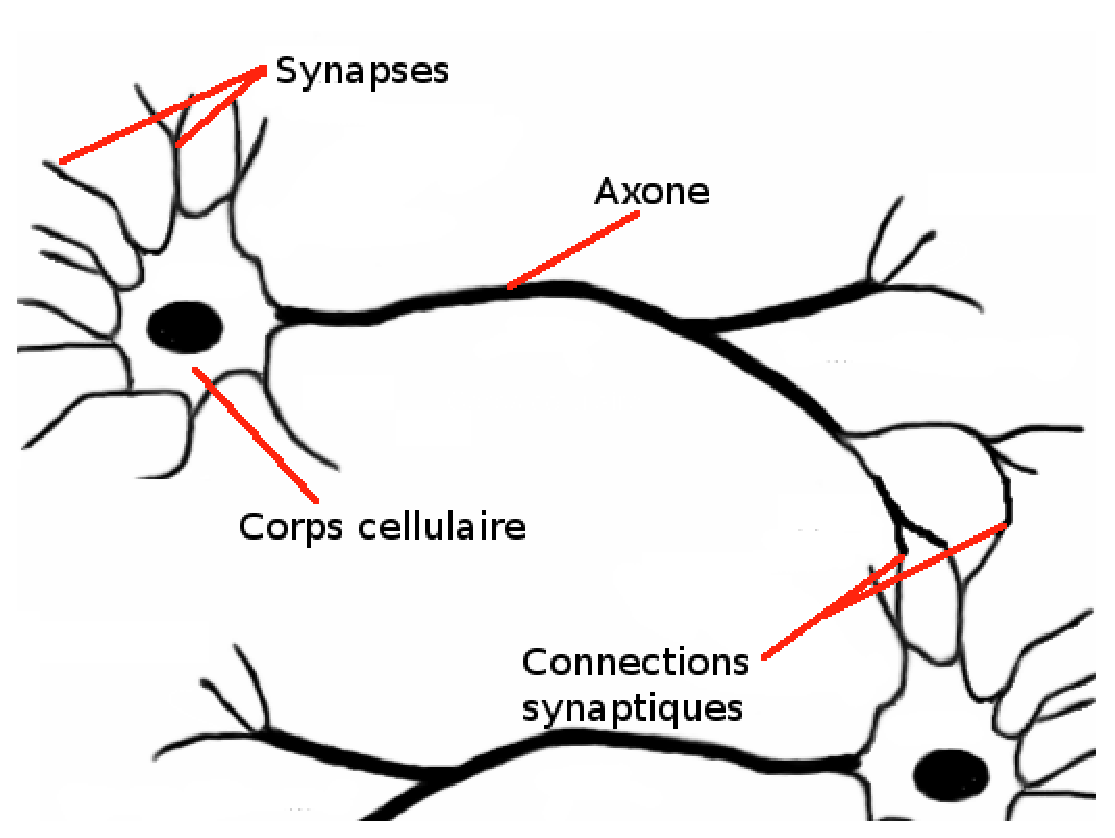
\includegraphics[width=8cm]{predoc/images/neurone-bio.eps}
\end{center}
\caption{\label{fig:neurobio} Schéma de deux neurones, l'un connecté à l'autre}
\end{figure}

\subsubsection{Copier le cerveau?}

L'idée de copier le cerveau à l'aide de réseaux de neurones artificiels est
assez présomptueuse et cela ne nous concerne pas. On s'inspire seulement de
l'hypothèse d'architecture "connectionniste" du cerveau pour bâtir des réseaux
de neurones artificiels, avec notamment cette idée que le réseau de neurones
artificiel soit composé de plusieurs couches d'un degré de complexité toujours
plus élevé.

Même s'il est aussi possible d'utiliser les dernières avancés en neurosciences
pour affiner des algorithmes déjà existants \cite{lowe}\footnote{\textbf{Jim
Mutch and David G. Lowe}, \textit{Object class recognition and localization
using sparse features with limited receptive fields}, International Journal of
Computer Vision, 80, 1 (2008), pp. 45-57.}, notre objectif premier reste celui
de concevoir un modèle qui puisse automatiquement apprendre à exécuter avec
succès une tâche particulière (classification, régression,...). En aucun cas
nous ne cherchons à comprendre le fonctionnement du cerveau au travers
d'interprétations de nos modèles!

Concernant la recherche sur le fonctionnement du cerveau, on pourra citer la
collaboration d'IBM et de l'École Polytechnique de Lausanne pour le Blue Brain
Project\footnote{http://bluebrain.epfl.ch/} qui a réussi en 2006 à reproduire
une colonne corticale du cerveau à partir d'un amas de données considérable.
Aussi pour affûter notre curiosité, cette expérience réussie de simulation de
pilotage d'un avion de chasse F-22 par $25 000$ neurones extraits du cortex
cérébral moteur d'embryons de rats\footnote{voir site de Thomas DeMarse}.

\subsection{Historique des Réseaux de Neurones Artificiels}


Afin de décrire ce qu'est un réseau de neurones artificiel, on commence par
l'unité de base du réseau: le neurone artificiel.

\subsubsection{Neurone formel}

En 1943, Warren McCulloch et Walter Pitt \cite{macculloch}\footnote{\textbf{W.
McCulloch, W. Pitt},\textit{A logical calculus of the ideas immanent in nervous
activity}, Bulletin of Mathematical Biology, pages 115-133, 1943} introduisent
le premier modèle de neurone formel afin d'étudier et de tenter d'élucider le
fonctionnement de notre système cérébral. Ce modèle mathématique de neurone
(voir figure \ref{fig:neuroformel}) effectue une somme pondérée de ses entrées
$X\in\mathbb{R}^{n}$ et transforme le résultat via une \textbf{fonction
d'activation} $f$, donnant ainsi la sortie du neurone. La somme pondéree par
les poids $w_{i}$ en entrée définit le niveau d'activation du neurone. Le biais
$b$ définit le seuil d'activation du neurone. En effet, si le niveau
d'activation d'un neurone dépasse son seuil d'activation, alors l'argument de
la fonction d'activation - ici la fonction de \textit{Heaviside} - devient
positif: le neurone est considéré comme étant actif. On a donc:

\begin{equation}
f(x)=\left\{\begin{array}{ll}
1 & \textrm{si }  \sum_{i=1}^{n}w_{i}x_{i}>b\\
0 & \textrm{sinon} \\
\end{array}\right.
\end{equation}

\begin{figure}
\begin{center}
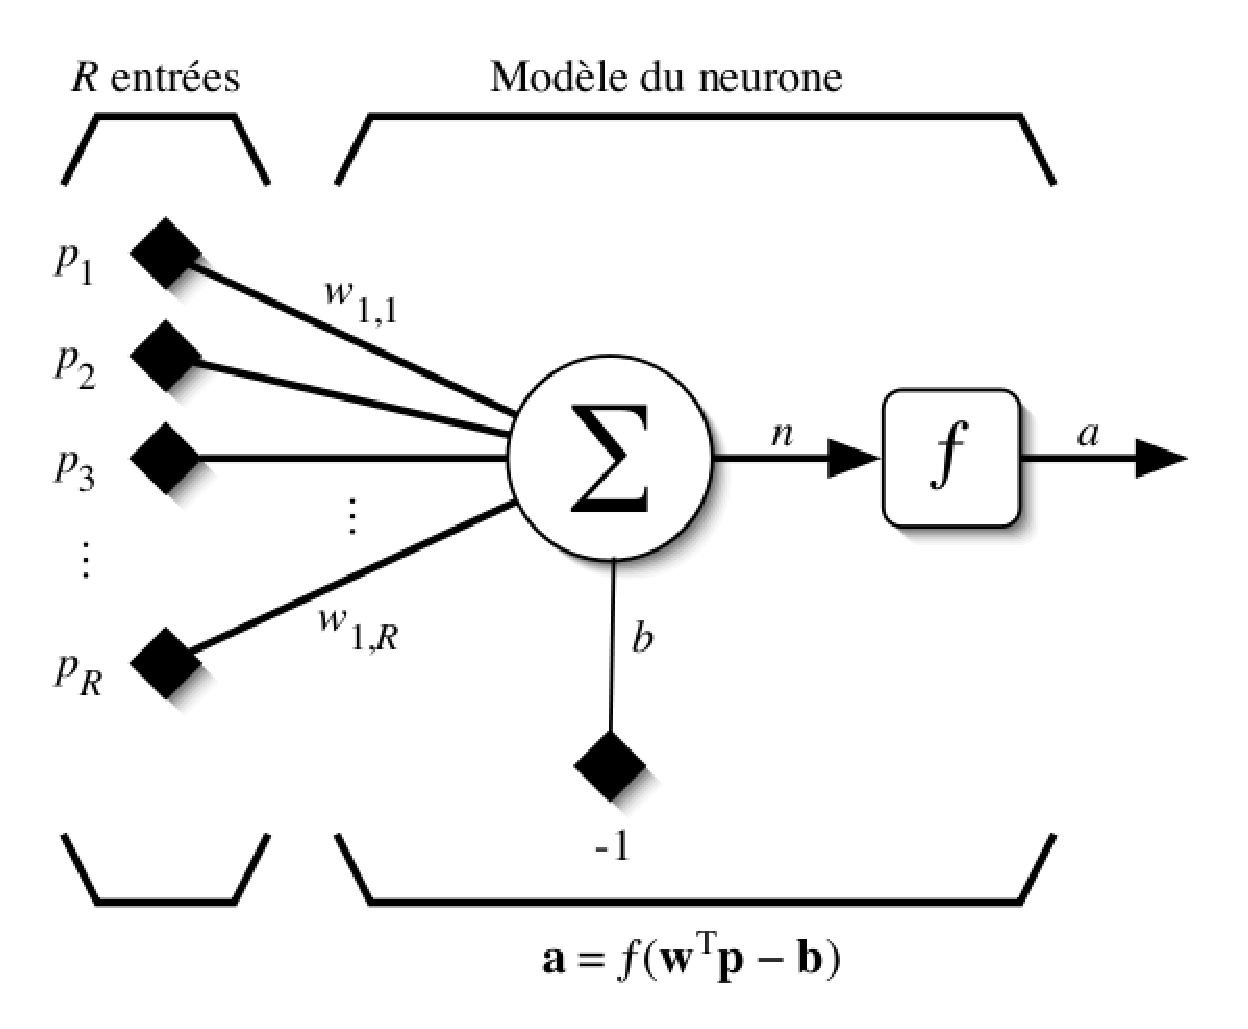
\includegraphics[width=6cm]{predoc/images/neurone_artificiel.eps}
\end{center}
\caption{\label{fig:neuroformel} Neurone artificiel, modifié depuis \cite{parizeau}.}
\end{figure}


En connectant ces unités simples les unes aux autres, il devient alors possible
de créer des réseaux de neurones artificiels. La première ébauche d'un modèle
de réseau de neurones artificiel est celle du Perceptron simple inventé par
Frank Rosenblatt en $1958$.

\subsubsection{Perceptron simple}

Le Perceptron simple est une architecture à propagation vers l'avant à une
seule couche cachée composée de plusieurs neurones. Par propagation vers
l'avant, on entend que tous les neurones d'une couche possèdent une connection
orientée vers chaque neurone de la couche suivante. Les neurones d'une même
couche ne sont pas connectés entre eux.

\textbf{\underline{Définition:}} Un perceptron à $m$ neurones est une fonction
de $\mathbb{R}^{n}$ dans $\lbrace 0,1\rbrace^{m}$. Il est caractérisé par
$m(n+1)$ paramètres: la matrice de poids $W\in\mathbb{R}^{m\times n}$ et le
biais $b\in\mathbb{R}^{m}$ avec $n$ la dimension de l'entrée.

\begin{figure}
\begin{center}
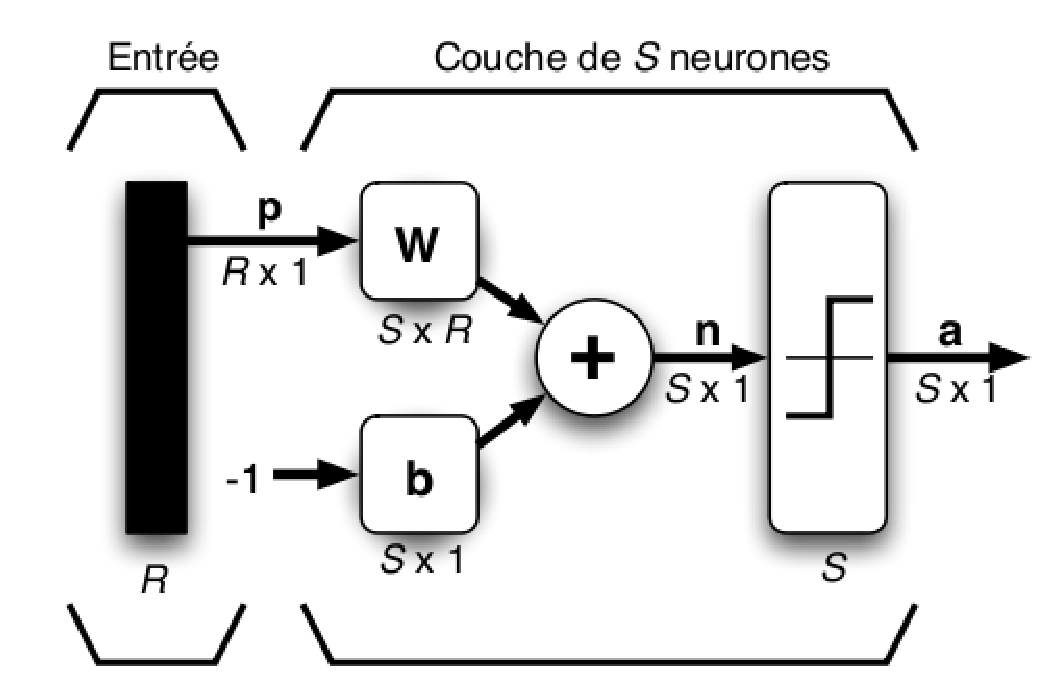
\includegraphics[width=6cm]{predoc/images/percep.eps}
\end{center}
\caption{\label{fig:percep} Perceptron, modifié depuis \cite{parizeau}.}
\end{figure}

L'idée géométrique du perceptron est de séparer l'ensemble des données à l'aide
d'un hyperplan.

\subsubsection{Apprentissage}

La règle d'apprentissage du Perceptron simple est inspirée de la règle de
Donald Hebb énoncée en 1949:

\textit{"When an axon of cell A is near enough to excite a cell B and
repeatedly or persistently takes part in firing it, some growth process or
metabolic changes take place in one or both cells such that A’s efficiency as
one of the cells firing B, is increased."}

Si deux neurones sont activés pour le même vecteur d'entrée, cela renforce la
connection qui les unie. Il devient alors possible de s'en inspirer pour
entraîner un Perceptron simple. On considère chaque composante du vecteur
d'entrée comme un neurone appartenant à la couche d'entrée. Puis on procède à
l'apprentissage de notre modèle en prenant en compte les activations
simultanées des neurones de la couche d'entrée et de la couche cachée.

\begin{itemize}
\item \textbf{Initialisation} des paramètres $\lbrace W,b\rbrace$ à des valeurs aléatoires.
\item \textbf{Tant que} l'ensemble d'apprentissage $S=\lbrace(x^{(i)},y^{(i)})\in\mathbb{R}^{n}\times\lbrace 0,1\rbrace^{m}\rbrace_{i=1,\dots ,n}$ n'est pas entièrement classifié correctement:
\begin{list}{}{}
\item \textbf{Pour} chaque neurone $1\leq j\leq m$:
\begin{enumerate}
\item Si le perceptron prédit la bonne valeur de sortie $y_{k}$, on ne fait rien.
\item Si le perceptron se trompe, on modifie la ligne correspondante $W_{k.}$ de la matrice de poids et la composante $b_{k}$ du biais :
\begin{itemize}
\item Si $y_{k}=1$ on procède à un \textbf{renforcement} des connections:
\begin{eqnarray}
\left\{\begin{array}{ll}
W_{k.} &\leftarrow W_{k.} + x_{k}\\
b_{k} &\leftarrow b_{k} + 1\\
\end{array}\right.
\end{eqnarray}
\item Si $y_{k}=0$ on procède à une \textbf{inhibition} des connections:
\begin{eqnarray}
\left\{\begin{array}{ll}
W_{k.} &\leftarrow W_{k.} - x_{k}\\
b_{k} &\leftarrow b_{k} - 1\\
\end{array}\right.
\end{eqnarray}
\end{itemize}
\end{enumerate}
\end{list}
\end{itemize}

Dans \cite{percep_converge}\footnote{\textbf{F. Rosenblatt}, \textit{Principles
of Neurodynamics}, Spartan Books, Washington D.C., 1962, 111–116}, F.
Rosenblatt présente un théorème qui garantit la convergence de l'algorithme
précédent sous l'hypothèse que les données de l'ensemble d'apprentissage soient
linéairement séparables. Malheureusement, le problème considéré ici n'est pas
mathématiquement bien posé.

En effet, un problème est dit bien posé au sens de Hadamard si:

\begin{enumerate}
\item la solution existe
\item la solution est unique
\item la solution est stable \textit{id est} robuste à de faibles perturbations de l'entrée.
\end{enumerate}

Certes, le théorème nous assure que la solution existe. Cependant, sauf pour
certains cas particuliers, il existe une infinité d'hyperplans qui peuvent
séparer l'ensemble d'apprentissage (zone verte de la figure
\ref{fig:percep_g}). La solution n'est donc pas unique. De plus, si on ajoute
un nouvel exemple à l'ensemble d'apprentissage, la solution est susceptible de
changer. En effet, si l'hyperplan solution est trop proche des vecteurs
d'apprentissage, la solution n'est pas stable.

\begin{figure}[!h]
\begin{center}
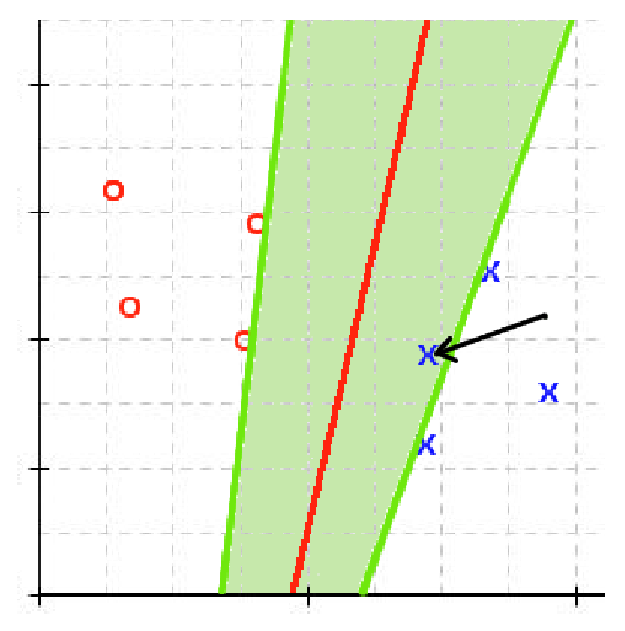
\includegraphics[width=6cm]{predoc/images/percep_graph2.eps}
\end{center}
\caption{\label{fig:percep_g} Ensemble des solutions de la règle d'apprentissage du perceptron. Un exemple a été rajouté (voir flèche) pour montrer que la solution n'est pas robuste. On préfèrerait avoir une solution semblable à la droite rouge.}
\end{figure}

Afin de palier à cette tendance à coller les données de l'ensemble
d'apprentissage, on introduit dans la section suivante un nouveau modèle et
ainsi que sa règle d'apprentissage basée sur la minimisation de l'erreur
quadratique moyenne.

\subsubsection{ADALINE et méthode des moindres carrés\label{adaline}}

Créé en 1960 par Bernad Widrow et Ted Hoff, ADALINE
\cite{adaline}\footnote{\textbf{B. Widrow, T. Hoff}, \textit{Adaptive switching
circuits}, 1960 Institute of Radio Engineers, Western Electronic Show, IRE
WESCON Convention Record} (pour \textit{ADApatative LInear NEuron}) est un
réseau de neurone à une couche cachée composée de $m$ neurones (voir figure
\ref{fig:adaline}).  \\

La différence avec le Perceptron simple réside dans la fonction d'activation
qui est ici purement linéaire \textit{id est} $f(x)=x$. Aussi la régle
d'apprentissage pour ce type de réseau de neurones est différente: il s'agit de
la méthode des moindres carrés (Least Mean Square).

\begin{figure}[!h]
\begin{center}
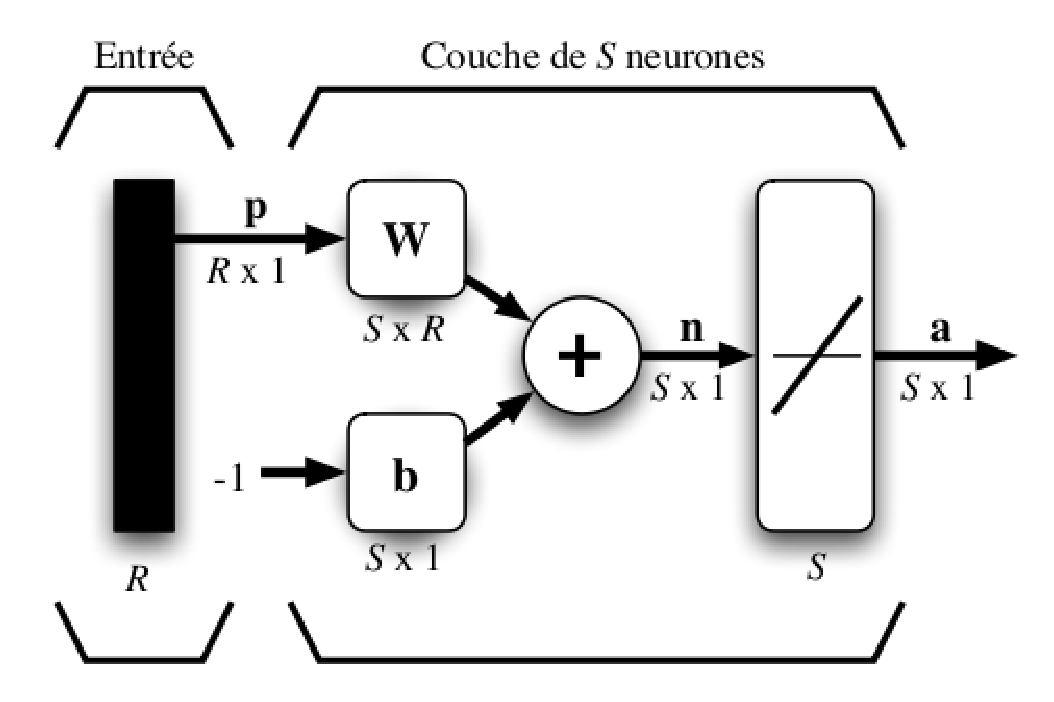
\includegraphics[width=8cm]{predoc/images/adaline.eps}
\end{center}
\caption{\label{fig:adaline} Réseau ADALINE, modifié depuis \cite{parizeau}}
\end{figure} 

La sortie du réseau ADALINE associé à l'entrée $X$ est donnée par:

\begin{eqnarray}
F_{W,b}(X) =  WX -b
\end{eqnarray}

La distribution des vecteurs d'entrée $X$ étant inconnue, on ne peut pas
calculer l'espérance de l'erreur de classification ($Y$ discret) ou de
régression ($Y$ continu). Pour un ensemble d'aprentissage
$S=\lbrace(X^{(i)},Y^{(i)})\in\mathbb{R}^{n}\times\mathbb{R}^{m}\rbrace_{i=1,\dots
,n}$, on estime cette espérance par l'erreur quadratique empirique moyenne
définie par:

\begin{eqnarray}
\hat{E}(W,b)=\sum_{i=1}^{n}\Vert F_{W,b}(X^{(i)})-Y^{(i)}\Vert^{2}_{2}
\end{eqnarray}

Plutôt que de calculer l'erreur moyenne pour l'ensemble d'apprentissage dans sa
totalité et de minimiser cete erreur par une descente de gradient, on estime
l'erreur quadratique moyenne par l'erreur quadratique pour un exemple donné.
Puis on procède à une minimisation par une descente de gradient stochastique
(décrit en section \ref{gradsto}). On a les gradients suivants:

\begin{eqnarray}
\frac{\partial}{\partial W}\hat{E}_{W,b}(X^{(i)},Y^{(i)}) = 2(WX^{(i)}-b-Y^{(i)})(X^{(i)})^{T}\\
\frac{\partial}{\partial b}\hat{E}_{W,b}(X^{(i)},Y^{(i)})  = 2(WX^{(i)}-b-Y^{(i)})
\end{eqnarray}

Dans le cadre de l'ADALINE, la surface d'erreur est quadratique. Concernant le
pas de gradient $\eta$, on peut démontrer que la convergence de la descente de
gradient est assurée pour un pas $0<\eta<\frac{1}{\lambda_{max}}$ où
$\lambda_{max}$ désigne la plus grande des valeurs propres de la Hessienne.

Contrairement à la solution donnée par la règle d'apprentissage du Perceptron
simple qui n'est pas optimale, souvent trop proche des patrons d'apprentissage
et donc sensible au bruit, la frontière se retrouve ici à égale distance des
deux classes (droite rouge de la figure \ref{fig:percep_g}) dans le cas
linéairement séparable. Si le problème n'est pas linéairement séparable, la
solution reste raisonnable dans la plupart des cas.

Si la régle LMS nous permet d'obtenir une frontière plus robuste au bruit que
la règle du perceptron, il n'en reste pas moins que toutes les solutions
trouvées par ADALINE ou le Perceptron simple sont des hyperplans. Pour le
moment, nous restons donc limités aux problèmes séparables par une simple
frontière linéaire pour ADALINE et aux problèmes linéairement séparables pour
le Perceptron simple.

\subsubsection{Limitations}

En plus de ces restrictions, le livre \textit{Perceptrons}
\cite{minsky}\footnote{\textbf{M. Minsky, S. Papert}, \textit{Perceptrons, An
Introduction to Computational Geometry}, MIT Press, Cambridge, Mass., 1969} de
Marvin Minsky et Seymour Papert sonne le glas pour les réseaux de neurones en
1969. Ils s'attaquent au Perceptron simple en utilisant les mathématiques
modernes comme la topologie et la théorie des groupes. Par une étude théorique
complète, ils décrivent les limitations du Perceptron simple et mettent en
évidence sa faible capacité.

Surtout, ils énoncent dans la continuité de leurs démonstrations la conjecture qu'un Perceptron multi-couches souffrirait des mêmes limitations du Perceptron simple:

\textit{"There is no reason to suppose that any of these vicues carry over the
many layered version. Nevertheless, we consider it to be a important research
problem to elucidate (or reject) our \underline{intuitive} judgement is
sterile."}(p.$231$)\cite{minsky} \\

Cette conjecture a été très mal interprétée et a provoqué l'arrêt des financements de la recherche sur ces modèles.

Voici quelques exemples de problèmes que les méthodes évoquées précedemment ne peuvent pas résoudre: les deux lunes et le OU exclusif "XOR".

\begin{figure}
\begin{center}
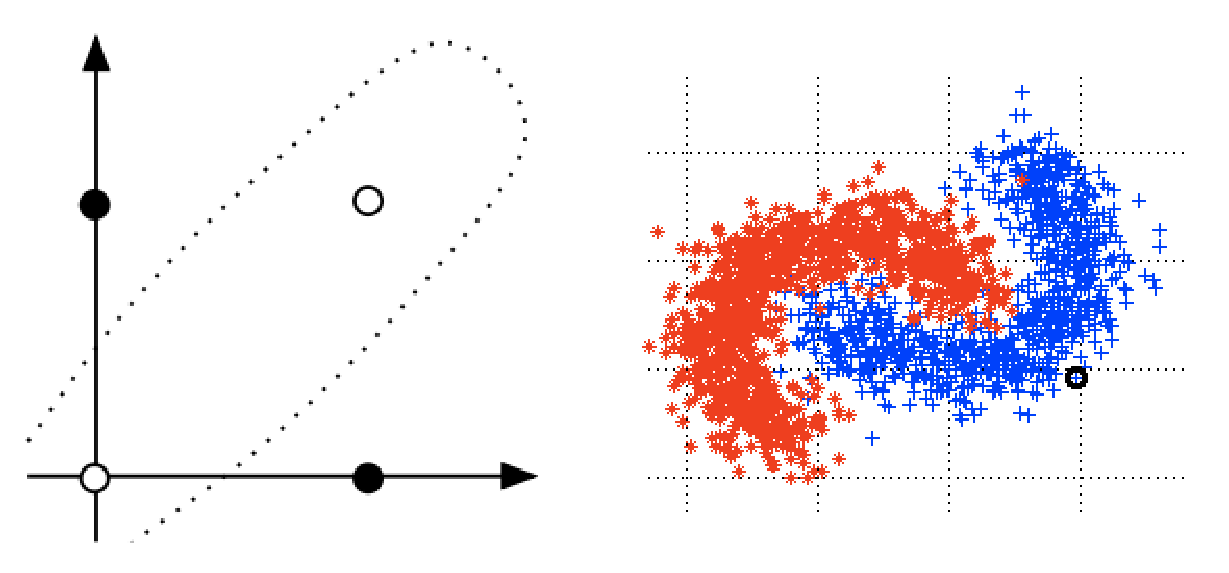
\includegraphics[width=9cm]{predoc/images/xor2moons.eps}
\end{center}
\caption{\label{fig:robustpercep} Problèmes non linéairement séparables}
\end{figure}


Pourtant la solution pour gagner en capacité semble résider dans l'augmentation
du nombre de couches du réseau. On notera que le fait d'assembler entre elles
plusieurs couches de types ADALINE donnera toujours un réseau équivalent à
l'ADALINE à une seule couche. On s'intéresse donc au Percetron multi-couches.

\subsubsection{Perceptron multi-couches}

L'idée du Perceptron multi-couches est de concaténer plusieurs Perceptrons
simples où la sortie d'une couche correspondrait à l'entrée de la couche
suivante (voir figure \ref{fig:percep_multicouche}).

\begin{figure}[!h]
\begin{center}
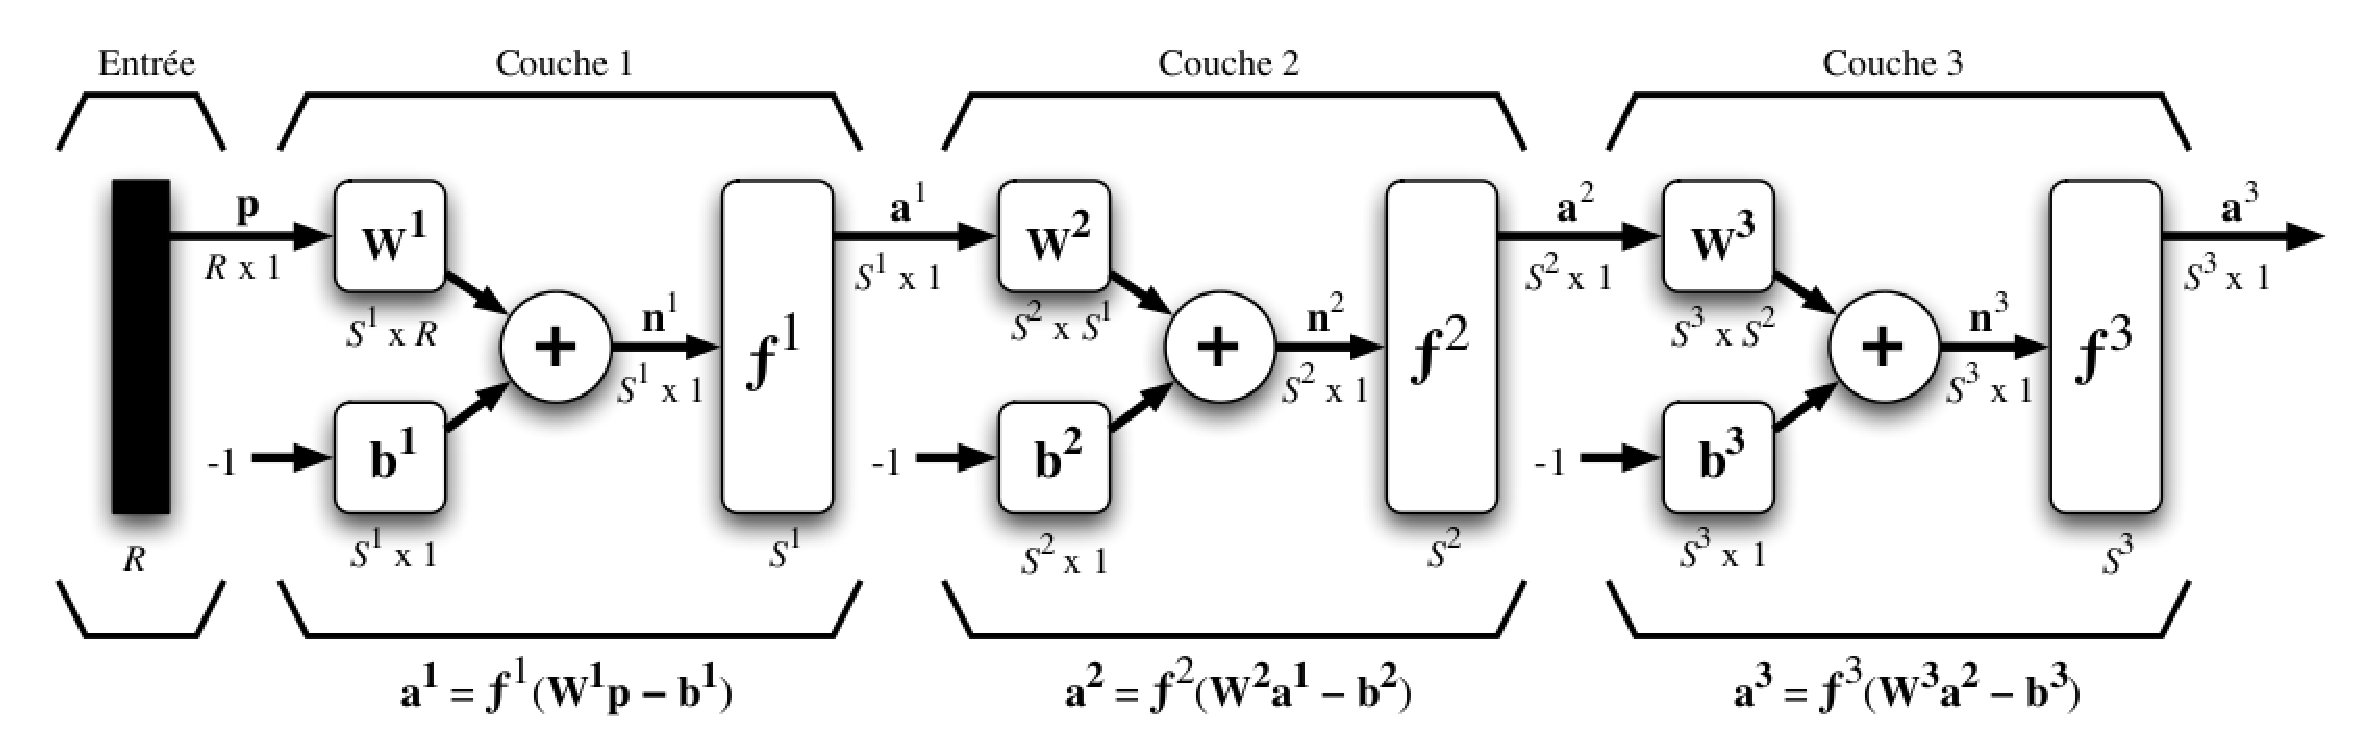
\includegraphics[width=12cm]{predoc/images/percep_multi.eps}
\end{center}
\caption{\label{fig:percep_multicouche} Architecture du Perceptron multi-couches, modifié depuis \cite{parizeau}}
\end{figure}

On peut constater que l'on gagne en capacité. En effet, un Perceptron à deux
couches peut résoudre le problème du OU exclusif (voir figure
\ref{fig:solvexor}). 

\begin{figure}[!h]
\begin{center}
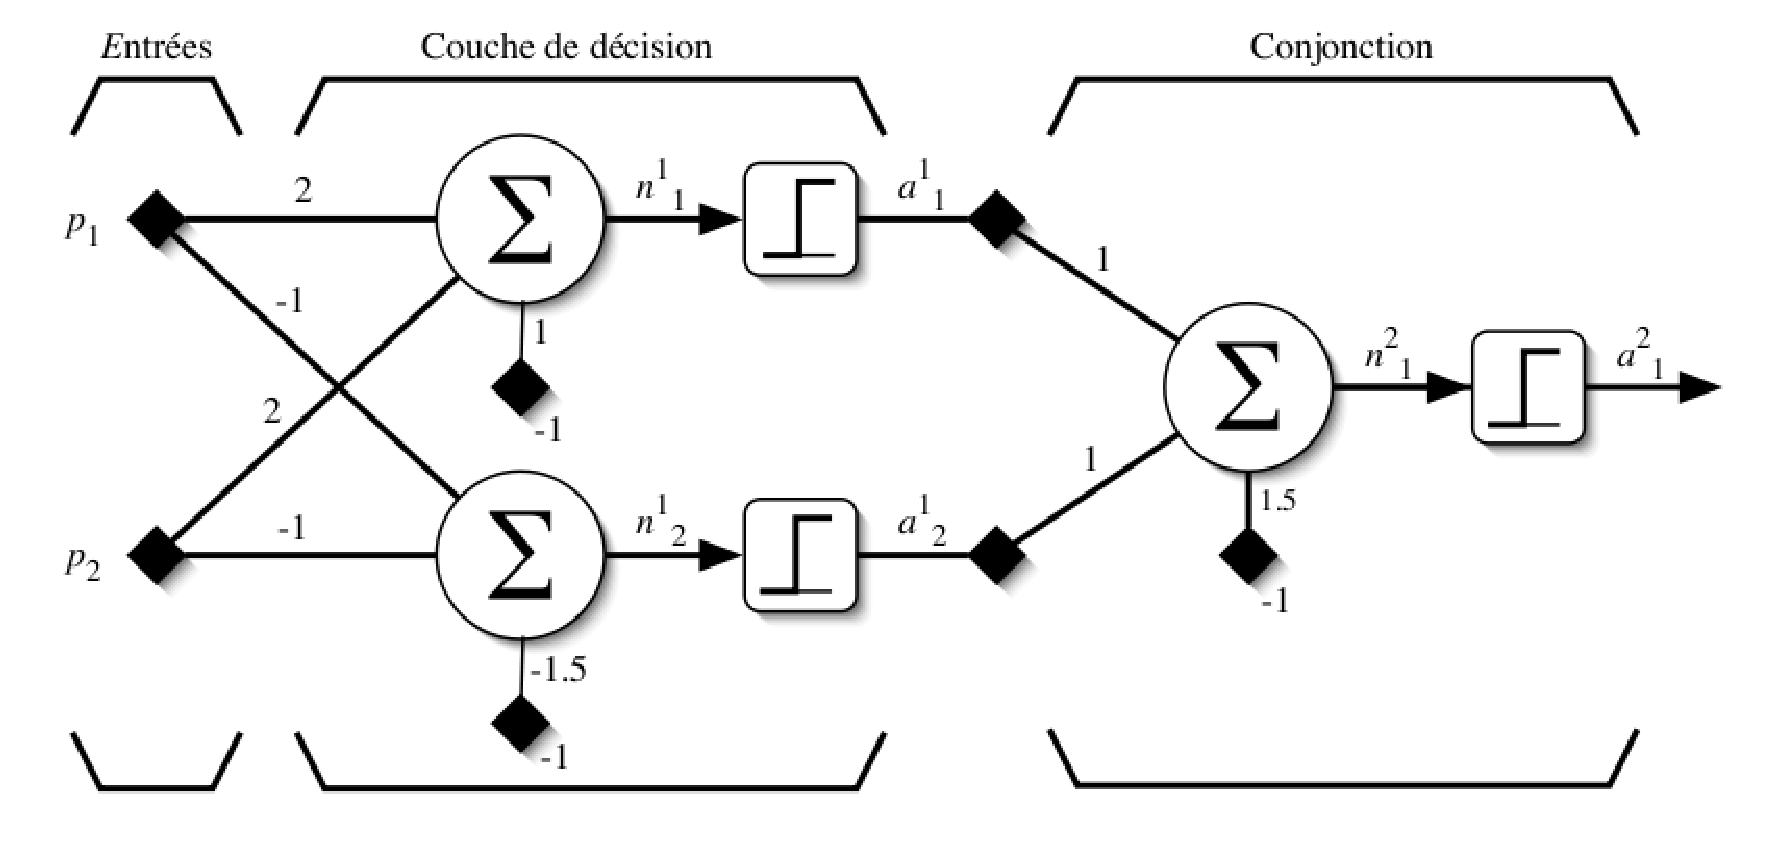
\includegraphics[width=6cm]{predoc/images/solvexor.eps}
\end{center}
\caption{\label{fig:solvexor} Perceptron multicouche construit manuellement qui résoud le problème XOR, modifié depuis \cite{parizeau}}
\end{figure}

\subsubsection{Frontières de décision}

Lorque l'on concatène plusieurs couches, on crée des combinaisons de frontières
de décision. Dans le cas des unités seuil, chaque neurone correspond à un
hyperplan. Ce qui nous donne les combinaisons de frontières de décision
illustrées en figure \ref{fig:frontieres}.

\begin{figure}[!h]
\begin{center}
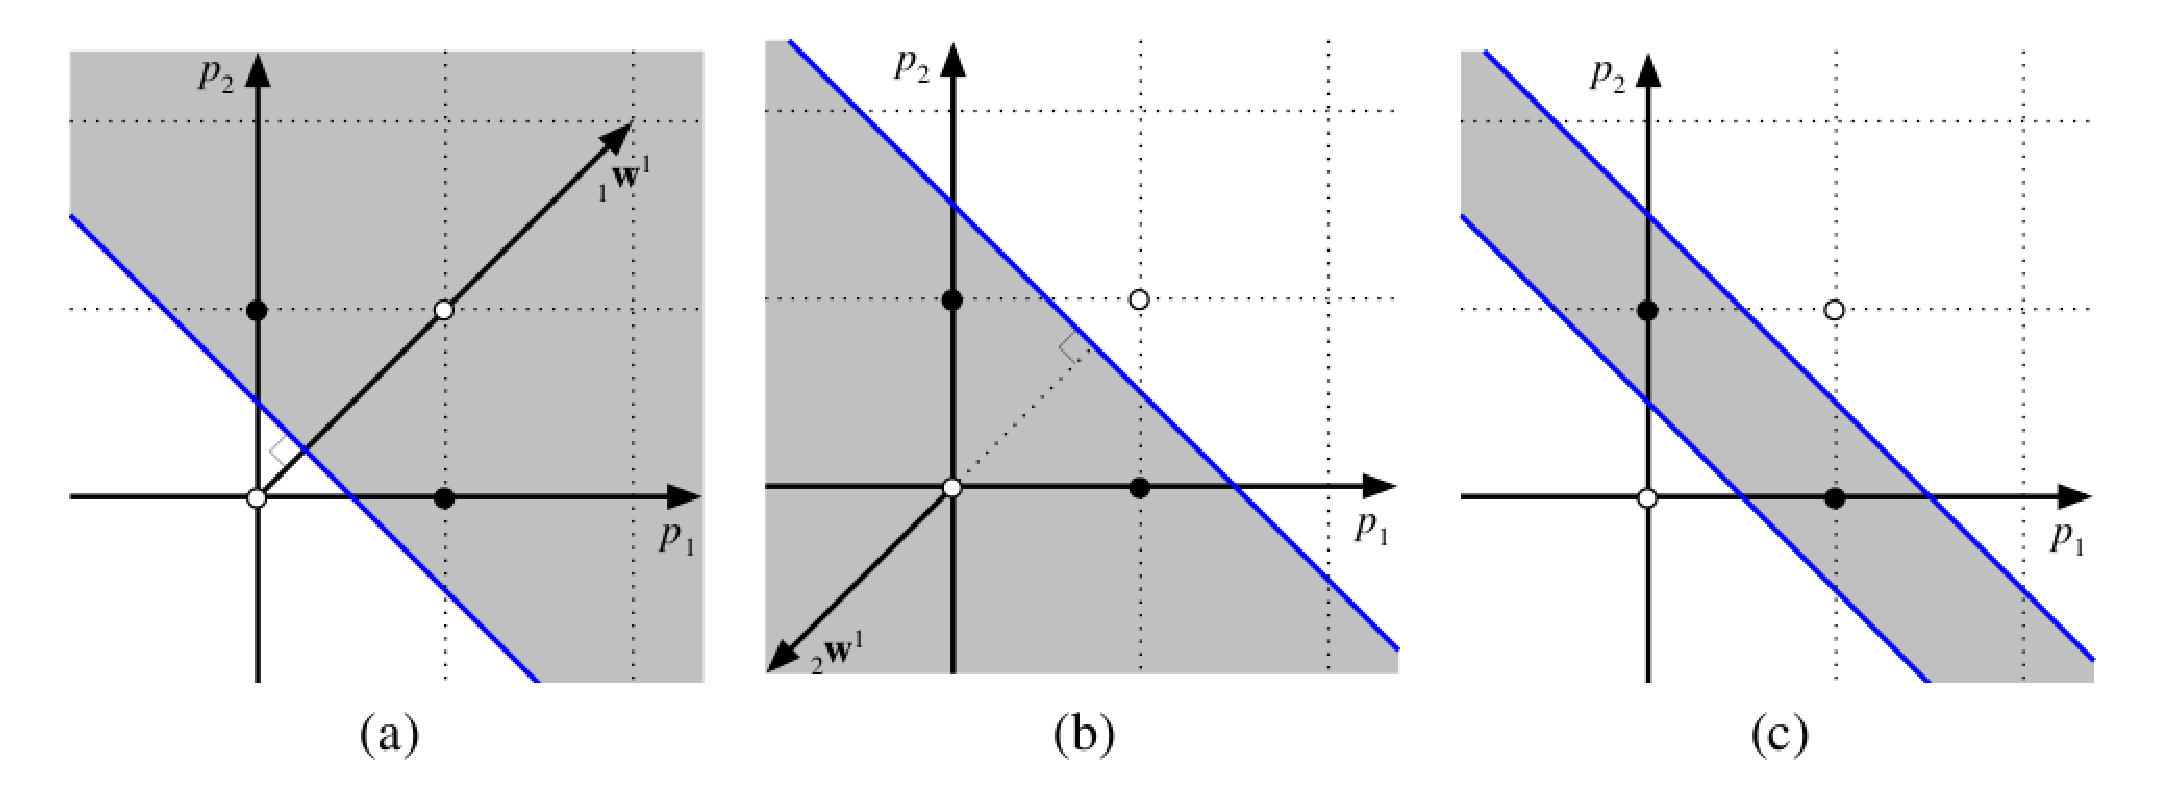
\includegraphics[width=8cm]{predoc/images/frontieres.eps}
\end{center}
\caption{\label{fig:frontieres} Frontières de décision engendrées par le réseau de la figure \ref{fig:robustpercep}, modifié depuis \cite{parizeau}. (a) et (b) correspondent aux frontières générées par les deux neurones de la première couche, (c) représente la conjontion de ces deux frontières réalisée par le neurone de la couche supérieure.}
\end{figure}

Si on utilise des fonctions d'activations non linéaires ($\tanh$ par exemple),
il devient alors possible d'obtenir des frontières de décisions non linéaires
pour chaque neurone: on peut modéliser des frontières de plus en plus complexes
définissant des ensembles convexes, concaves, ouverts, fermés.

\subsubsection{Théorème d'approximation universelle \label{univ}}

En 1989, George Cybenko donne la preuve du théorème d'approximation universelle
\cite{universelle}\footnote{\textbf{G Cybenko}, \textit{Approximation by
superpositions of a sigmoidal function}, Mathematics of Control, Signals, and
Systems (MCSS), 1989, Springer}. Ce théorème démontre qu'il est possible
approximer n'importe quelle fonction (avec une précision arbitraire) à l'aide
d'un réseau de neurones particulier à condition d'avoir suffisamment d'unités
dans la première couche cachée. Ce réseau (illustré en figure \ref{fig:approx})
est composé d'une couche de fonctions d'activation de type sigmoïde
$f(x)=1/(1+e^{-x})$ et d'une seconde couche linéaire. Plus simplement, il est
démontré que toute fonction peut être approximée par une combinaison linéaire
de sigmoïdes.  \\

\begin{figure}[!h]
\begin{center}
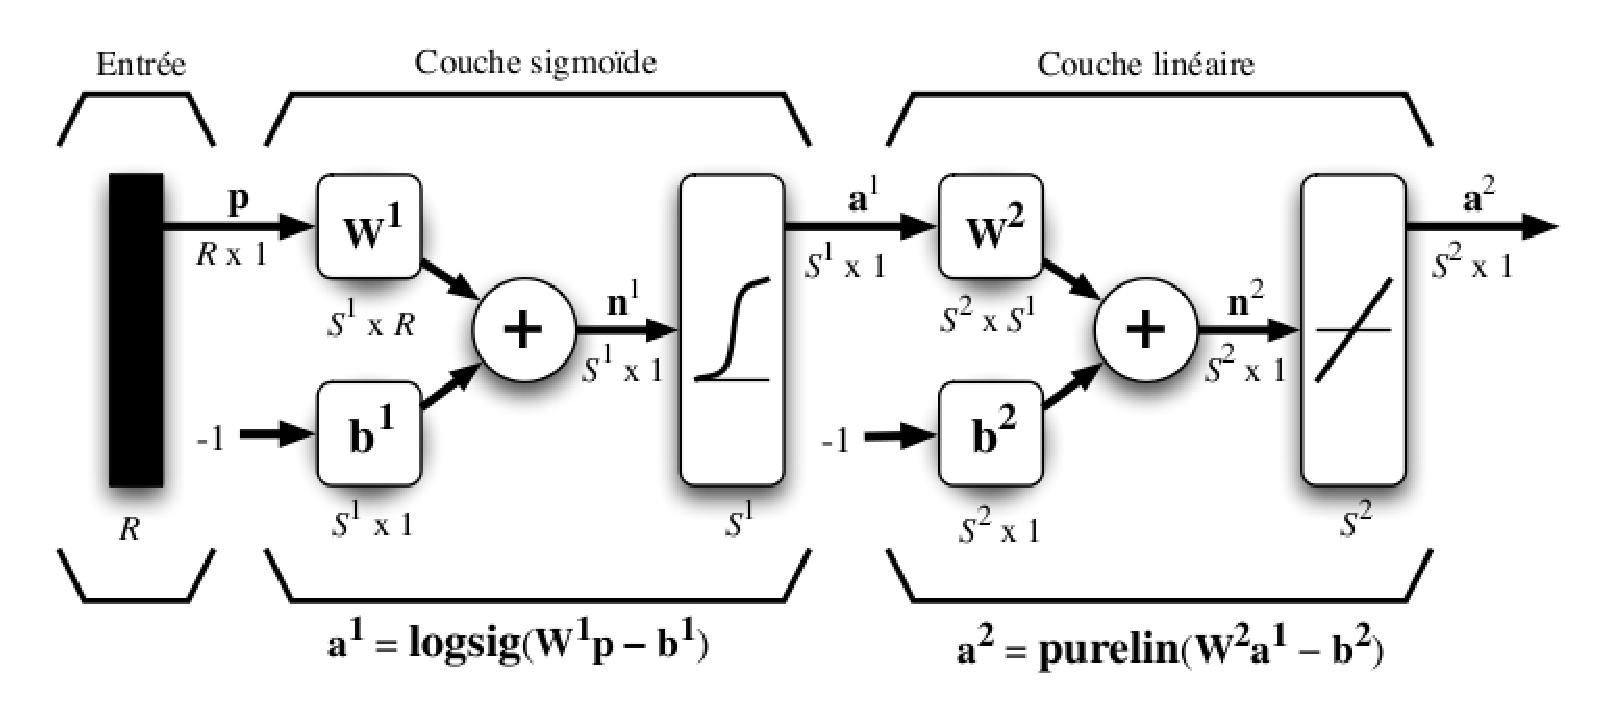
\includegraphics[width=8cm]{predoc/images/approx.eps}
\end{center}
\caption{\label{fig:approx} Réseau de neurones pour l'approximation de fonctions, modifié depuis \cite{parizeau}}
\end{figure}

\subsubsection{Méthode d'apprentissage}

Avant 1985-86, on ne disposait pas de régle d'apprentissage viable pour
entraîner ces réseaux de neurones multi-couches. L'idée première est d'utiliser
la règle LMS pour un Perceptron simple. Il faut donc remplacer la fonction
d'activation \textit{Heaviside} qui n'est pas différentiable par une fonction
de type sigmoïde. Puis on généralise cette règle pour le cas des Perceptrons
multi-couches en rétro-propageant l'erreur dans les couches inférieures. Il
aura fallu attendre l'arrivée de l'algorithme de rétro-propagation
\cite{rumel}\footnote{\textbf{D. Rumelhart, R. Williams, G. Hinton},
\textit{Learning internal representations by error propagation}, chap 8,
Parallel distributed processing, 1986} pour que l'on soit en mesure d'entraîner
ces réseaux de neurones.

TODO RETROPROP

\subsubsection{Comment entraîner un réseau de neurones?}



\section{Apprentissage non supervisé de représentations}

L'apprentissage non supervisé permet d'extraire des connaissances sur des
données sans connaissance à priori. On ne connaît ni le type des données
\textit{e.g.} musique, images, données séquentielles, ni leur classe
d'appartenance \textit{e.g.} $10$ classes de $0$ à $9$ pour la classification
de chiffres.  \\

Il est très difficile de savoir pourquoi un algorithme d'apprentissage non
supervisé fonctionne (bien ou mal) sur un certain type de données.  De manière
non exhaustive, voici énumérés quelques-uns des facteurs qui rendent difficile
une analyse complète du fonctionnement de ces algorithmes: haute
dimensionnalité des données, mauvais conditionnement du problème
d'optimisation, processus d'optimisation non convexe, nombreuses
paramétrisations possibles des modèles...  \\

Une manière usuelle de sélectionner les hyper-paramètres de tels algorithmes passe 
par une évaluation des performances discriminatives de la
représentation apprise.

On présente ici la méthode linéaire la plus courante et la plus populaire:
l'analyse en composantes principales ou en anglais \textit{Principal Component
Analysis} \textbf{(PCA)}~\cite{Pearson-1901,Hotelling1933}.

\subsection{Analyse en Composantes Principales} \label{sec:pca}

Une PCA avec $k$ composantes principales permet d'obtenir les $k$ composantes
orthonormales dans l'espace d'entrée sur lesquelles projeter les données telles
que l'on retient le plus de variance dans les données. Ces composantes
correspondent aux premiers vecteurs propres (si on les ordonne par valeurs
propres décroissantes) de la matrice de covariance des données.  Ces
composantes sont ordonnées: la première correspond à la direction qui retient
le plus d'information et ainsi de suite par niveau de variance décroissant.

\paragraph{Algorithme} Soit $X\in\mathcal{M}_{n\times d}(\mathbb{R})$ la
matrice qui contient l'ensemble d'entraînement $\mathcal{D}=\lbrace
x^{(i)}\in\mathbb{R}^d \rbrace_{i=1,\dots,n}$.  En premier lieu, on calcule la
moyenne empirique $\mu=(1/n)\sum_{i=1}^{n}X_i$ où $X_i$ représente la ligne $i$
de la matrice X \textit{i.e.} l'exemple $i$. Les données sont centrées
$\tilde{X}=X-\mu$ et on calcule la matrice de covariance
$C=(1/n)\tilde{X}^T\tilde{X}$. La décomposition en valeurs propres de $C$ est
ensuite calculée (la partie la plus co\^uteuse): $C=V^{-1}UV$ où
$U$ est une matrice diagonale qui contient l'ensemble des valeurs propres
et $V\in\mathcal{M}_{d\times d}$ les vecteurs propres associés (chaque colonne
correspond à un vecteur propre). La sortie de la PCA est alors donnée par:

\begin{equation}
Y=(X-\mu)V
\end{equation}

Si l'on veut avoir une PCA avec \textit{whitening}, on construit la matrice
diagonale $U^{'}$ à partir de $U$ où $U^{'}_{ii}=1/\sqrt{C_{ii}}$ et la sortie
est alors donnée par:

\begin{equation}
Y=(X-\mu)VU^{'}
\end{equation}


Suivant la dimension des données ou le nombre d'exemples d'entraînement, il
existe deux algorithmes différents qui permettent d'extraire en
$O(\min(n,d)^3)$~\cite{bishop-book2006}.  Le cube est dû à l'inversion de
matrice.

\paragraph{Hyper-paramètres} Les hyper-paramètres de la PCA comprennent le
nombre de composantes à garder pour la transformation (le nombre de colonnes de
$V$ à conserver) et le fait d'effectuer ou non du \textit{whitening}. Parfois,
les premières composantes contiennent une information utile tandis que les
dernières composantes représentent du bruit (voir Figure~\ref{fig:mnistpca}).


\begin{figure}
\centering
\begin{subfigure}{0.45\textwidth}
\begin{tabular}{c}
  \includegraphics[width=0.9\linewidth]{predoc/images/0_ppv.png}\\
  \includegraphics[width=0.90\linewidth]{predoc/images/1_ppv.png}\\
  \includegraphics[width=0.90\linewidth]{predoc/images/2_ppv.png}\\
  \includegraphics[width=0.90\linewidth]{predoc/images/3_ppv.png}\\
  \includegraphics[width=0.90\linewidth]{predoc/images/4_ppv.png}\\
  \includegraphics[width=0.90\linewidth]{predoc/images/5_ppv.png}\\
  \includegraphics[width=0.90\linewidth]{predoc/images/6_ppv.png}\\
  \includegraphics[width=0.90\linewidth]{predoc/images/7_ppv.png}\\
  \includegraphics[width=0.90\linewidth]{predoc/images/8_ppv.png}\\
  \includegraphics[width=0.90\linewidth]{predoc/images/9_ppv.png}
\end{tabular}
\label{fig:mnistppv}
\end{subfigure}
\begin{subfigure}{0.45\textwidth}
% \subfigure[$10$-pca components]{
\begin{tabular}{c}
  \includegraphics[width=0.9\linewidth]{predoc/images/0_eigenvectors.png}\\
  \includegraphics[width=0.90\linewidth]{predoc/images/1_eigenvectors.png}\\
  \includegraphics[width=0.90\linewidth]{predoc/images/2_eigenvectors.png}\\
  \includegraphics[width=0.90\linewidth]{predoc/images/3_eigenvectors.png}\\
  \includegraphics[width=0.90\linewidth]{predoc/images/4_eigenvectors.png}\\
  \includegraphics[width=0.90\linewidth]{predoc/images/5_eigenvectors.png}\\
  \includegraphics[width=0.90\linewidth]{predoc/images/6_eigenvectors.png}\\
  \includegraphics[width=0.90\linewidth]{predoc/images/7_eigenvectors.png}\\
  \includegraphics[width=0.90\linewidth]{predoc/images/8_eigenvectors.png}\\
  \includegraphics[width=0.90\linewidth]{predoc/images/9_eigenvectors.png}
\end{tabular}
\label{fig:mnistpca}
\end{subfigure}

   \caption{Sur MNIST, pour un exemple de chaque classe (chiffres de $0$ à $9$) on
   extrait les $10$ plus proches voisins (ppv) intra-classe et on entraîne une PCA sur cet
   ensemble. Les $10$ ppv sont présentés en Fig.~\ref{fig:mnistppv} et les
   composantes des $10$ différentes PCA en Fig.~\ref{fig:mnistpca}. Les premières composantes de
   la PCA contiennent des informations utiles (de possibles transformations)
   tandis que les dernières n'encodent que du bruit.}

\end{figure}


On s'intéresse ici à des méthodes qui peuvent être utilisées par la suite pour
l'initialisation de réseaux de neurones.
%(voir Section~\ref{sec:nn})
Depuis la formalisation la plus classique de l'auto-encodeur
\textbf{(AE)}~\cite{Gallinari87} , nous présenterons le \textit{Denoising
Auto-Encoder} \textbf{(DAE)}~\cite{VincentPLarochelleH2008,Vincent-JMLR-2010}.
%Après une analyse de l'effet du bruit utilisée lors du processus
%d'apprentissage,
Ensuite, nous présenterons le \textit{Contractive Auto-Encoder}
\textbf{(CAE)}~\cite{Rifai+al-2011,Salah+al-2011} et sa version la plus
sophistiquée le \textit{Higher-Order Contractive Auto-Encoder}
\textbf{(CAE+H)}~\cite{Salah+al-2011}.

\subsection{Architectures de type Auto-Encodeur}

L'auto-encodeur classique se décompose en un encodeur et un décodeur.
L'encodeur effectue une transformation affine des données paramétrisée par une
matrice de poids $W\in\mathcal{M}_{m\times d}(\mathbb{R})$ où $m$ désigne le
nombre d'unités cachées du modèle et un vecteur de biais $b\in\mathbb{R}^m$.
Cette transformation est suivie d'une non-linéarité $s:\mathbb{R}^m \rightarrow
\mathbb{R}^m$ appliquée à chaque élément du vecteur. En général, on utilise la
fonction logistique $s(x)=1/(1+e^{-x})$ mais la tangente hyperbolique est aussi
communément utilisée. On a donc la forme globale suivante:

\begin{equation}
h(x)=s(Wx+b)
\end{equation}

Le décodeur tente de reconstruire l'exemple $x$ à partir de la représentation
cachée $h(x)$ et peut partager en la m\^eme matrice de poids que l'encodeur
mais a un vecteur de biais $b^{'}\in\mathbb{R}^d$ qui lui est propre. Il a
alors la forme suivante:

\begin{equation}
r(x)=s(W^{T} h(x)+b^{'})
\end{equation} 

La non-linéarité $s(.)$ est ici optionnelle et dépend de la nature des données
ou de la sortie désirée du décodeur \textit{i.e.} si elle doit \^etre dans
l'intervalle $[0,1]$ ou non.  \\

\paragraph{Algorithme}
Tous ces paramètres sont ajustés par optimisation \textit{e.g.} descente de
gradient stochastique, visant à réduire l'erreur de reconstruction suivante:

\begin{equation}
\mathcal{J}_{\textrm{AE}} = \frac{1}{\vert \mathcal{D}\vert}\sum_{x\in\mathcal{D}}\mathcal{L}(x,r(h(x)))
\label{eq:ae}
\end{equation}

La fonction de perte $\mathcal{L}$ utilisée est en général, dans le cas de
données binaires (ou modélisant des probabilités), l'entropie croisée négative
$\mathcal{L}(x,y) = -\sum_{i=1}^d x_i\log y_i + (1-x_i)\log(1-y_i)$ ou la
\textit{Mean Squared Error} (MSE) $\mathcal{L}(x,y) = \| x-y\|^2_2$. Comme on
le verra par la suite à la Section~\ref{sec:perfs}, pour les fins
d'initialisation de réseaux de neurones de classification, les performances de
l'auto-encodeur classique sont largement dépassées par le DAE, CAE et CAE+H.

\paragraph{Hyperparamètres} Les hyperparamètres de ce genre d'architecture sont
malheureusement nombreux. En voici une liste non exhaustive et des exemples de
valeurs typiques à raffiner par une recherche des hyperparamètres optimaux: le
nombre d'unités cachées ($1,000$), la fonction d'activation de l'encodeur ou et
du décodeur (fonction sigmoide), la fonction de perte utilisée (MSE ou Entropie
croisée), le pas de gradient ($\lbrace 10^{-1},\dots,10^{-6}\rbrace$).  \\

Une fois une certaine expertise pratique acquise avec l'entraînement de ce genre
d'architectures, l'espace des hyperparamètres à explorer qui peut paraître
exponentiellement grand au premier abord peut se réduire à quelques valeurs.


\subsubsection{Auto-Encodeur Débruitant}

On présente ici l'Auto-Encodeur Débruitant, en anglais \textit{Denoising
Auto-Encoder} (DAE).  L'idée du DAE est qu'à partir de l'observation partielle
d'une entrée on doit être capable de reconnaître (reconstruire) l'entrée
originale. À un très haut niveau, on peut penser qu'en tant qu'êtres humains,
nous sommes capables de reconnaître des objets partiellement occultés ou aussi
bien à partir d'un son et d'une image, nous sommes en mesure de reconnaître un
film déjà vu en ne voyant que certaines séquences.  \\

Plutôt que de minimiser la perte classique Eq.~\ref{eq:ae}, on bruite l'entrée
$x$ et on force l'auto-encodeur à reconstruire l'entrée originale à partir de
la version bruitée $\tilde{x}$:

\begin{equation}
\mathcal{J}_{\textrm{DAE}} = \frac{1}{\vert \mathcal{D}\vert}\sum_{x\in\mathcal{D}}\mathcal{L}(x,r(h(\tilde{x})))
\label{eq:dae}
\end{equation}

Les processus de corruption communément utilisés sont le \textit{masking}
paramétré par $p$ la probabilité de mettre à zéro une composante de l'entrée ou
le bruit gaussien paramétré par $\sigma$ où $\tilde{x} = x + \epsilon$ où
$\epsilon \sim \mathcal{N}(0,\sigma)$. D'autres types de bruit
peuvent être utilisés (voir \cite{Vincent-JMLR-2010} pour une revue).

\paragraph{Hyperparamètres} On peut citer ici en plus des hyperparamètres de
l'auto-encodeur classique le type de bruit (gaussien ou \textit{masking}) et le niveau
de bruit.

%\section{Analyse de l'effet du bruit au cours de l'apprentissage}

%Différence entre DAE et CAE. Le DAE va avoir un décodeur qui est invariant à de
%petites variations de l'entrée. Sachant que seul l'encodeur est conservé pour
%l'entraînement de réseaux de neurones, il serait préférable d'avoir le encodeur
%qui soit invariant (CAE) et non pas le décodeur (DAE). 

\subsubsection{Auto-Encodeur Contractant}

On présente ici l'Auto-Encodeur Contractant, en anglais \textit{Contractive
Auto-Encoder}.
Contrairement à la PCA qui extrait les directions de variations
\textbf{globales} présente dans les exemples d'apprentissage, le CAE apprend
des directions de variations \textbf{locales}. Il suffit d'ajouter de manière
explicite dans la perte minimisée Eq.~\ref{eq:ae} une régularisation qui
correspond à la norme du jacobien de l'encodeur $h(x)$ par rapport à l'entrée
$x$ sur les points de l'ensemble d'entraînement $\mathcal{D}$:

\begin{equation}
\mathcal{J}_\textrm{CAE} = \mathcal{J}_\textrm{AE} + \lambda\frac{1}{\vert \mathcal{D}\vert}\sum_{x\in\mathcal{D}}\| \frac{\partial h}{\partial x}(x)\|_2^2
\label{eq:cae}
\end{equation}

Cette approche suggère aussi la possibilité de visualiser dans l'espace
d'entrée quelles sont les directions de variation autour d'un exemple
d'apprentissage auxquelles la représentation $h$ est sensible  (en regardant
les vecteurs propres du jacobien au point d'apprentissage). Cela permet
d'évaluer d'un point de vue qualitatif si l'extraction de caractéristiques a
convergé vers une solution intéressante ou non (voir Figure~\ref{fig:tan}).

\paragraph{Hyperparamètres} Contrairement au DAE, le CAE n'a ici qu'un seul
hyperparamètre en plus comparé à l'auto-encodeur classique. C'est le
coefficient de régularisation $\lambda$ ($0.1$ est un bon point de départ pour
chercher le coefficient optimal) qui va contrôler le compromis entre
erreur de reconstruction et invariance de la représentation.

\begin{figure}
\centering
\begin{subfigure}{0.9\linewidth}
%\subfigure[composantes d'une PCA sur CIFAR]
\includegraphics[width=0.9\linewidth]{predoc/images/pca.png}
\label{fig:tan_pca}
\end{subfigure}

\begin{subfigure}{0.9\linewidth}
%\subfigure[tangentes du CAE+H sur CIFAR]
\includegraphics[width=0.9\linewidth]{predoc/images/tangents_cifar.png}
\label{fig:tan_cifar}
\end{subfigure}

\begin{subfigure}{0.9\linewidth}
%\subfigure[tangentes du CAE+H sur MNIST]
\includegraphics[width=0.9\linewidth]{predoc/images/tangents_mnist.png}
\label{fig:tan_mnist}
\end{subfigure}


   \caption{ Sur MNIST et sur CIFAR (un ensemble d'predoc/images RGB), on présente les
   tangentes apprises par le CAE+H autour d'un point d'apprentissage en
   Figure~\ref{fig:tan_mnist},\ref{fig:tan_cifar}. On peut voir que ces
   tangentes encodent de l'information sur des transformation plausibles de
   l'image originale tandis que les composantes principales de la PCA n'ont
   encodé que du bruit (voir Figure~\ref{fig:tan_pca}). 
\label{fig:tan}}

\end{figure}





\subsubsection{Auto-Encodeur Contractant d'Ordre Supérieur}

Nous présentons ici une publication qui s'inscrit dans la recherche à laquelle j'ai contribué
au cours de mes deux premières années de doctorat \cite{Salah+al-2011}: il s'agit
de l'auto-encodeur contractant d'ordre supérieur, en anglais
\textit{Higher-order Contractive Auto-Encoder} (CAE+H).


Si le fait de pénaliser le premier ordre de la dérivée (jacobien) de l'encodeur
par rapport à l'entrée est bénéfique, il est naturel d'ajouter une pénalisation
concernant les ordres supérieurs (Hessien, troisième ordre, ...) au CAE
original (Eq.~\ref{eq:cae}). On pourra alors constater les effets obtenus en
termes de mesures quantitatives de performances de classification (bénéfique ou
non) ou de directions de variations obtenues (qualitatif).

Les pertes Eq.~\ref{eq:ae},~\ref{eq:dae} ou~\ref{eq:cae} sont minimisées par
descente de gradient. Il est donc nécessaire de pouvoir calculer les dérivées
partielles de la perte par rapport aux paramètres. Pour commencer, le calcul de
la $k^{\textrm{ième}}$ dérivée de l'encodeur (avec $m$ unités cachées) par
rapport à l'entrée (de dimension $d$) a une complexité algorithmique de
$O(md^k)$.  Calculer les dérivées partielles de cette dérivée par rapport aux
paramètres du modèles est donc prohibitif. Pour éviter ce calcul, on utilise
une approximation stochastique de la Hessienne (voir \cite{Salah+al-2011} pour
la preuve):

\begin{equation}
\|\dfrac{\partial^2 h}{\partial x^2}(x) \|_2^2 = \lim_{\sigma\rightarrow 0}\frac{1}{\sigma^2}\int_{\epsilon \rightsquigarrow \mathcal{N}(0,\sigma)} \| \dfrac{\partial h}{\partial x}(x) - \dfrac{\partial h}{\partial x}(x+\epsilon) \|^2_2 d\epsilon
\label{eq:hessian-approx}
\end{equation}

Si la variance $\sigma$ est non nulle, des contributions aux normes des ordres
supérieurs apparaissent \cite{Salah+al-2011}. Ces contributions disparaissent à
la limite $\sigma\rightarrow 0$. En pratique pour approximer la norme de la
Hessienne (Eq.~\ref{eq:hessian-approx}), on utilise un lot de plusieurs
versions bruitées $x+\epsilon$ du m\^eme exemple $x$ avec un $\sigma$ petit
mais non négligeable, ce qui donne lieu à l'approximation stochastique de la
norme de la Hessienne qui comporte aussi d'autres contributions provenant des
normes des ordres supérieurs (voir \cite{Salah+al-2011} pour plus de détails).

L'avantage d'utiliser cette approximation est que l'on peut pénaliser tous les
ordres supérieurs à moindre coût comparé à une complexité en $O(md^k)$.
L'inconvénient est de ne plus savoir exactement quels ordres sont pénalisés et
quelle est la contribution de chacun des ordres qui permet d'apprendre de
meilleures caractéristiques. Des expériences supplémentaires seront effectuées
sur des données de dimension réduite afin d'améliorer notre compréhension du
CAE+H.

En utilisant cette approximation,  on aboutit à la perte du \textbf{CAE+H} avec
une taille de lot $n_c$ et $\epsilon_i \rightsquigarrow \mathcal{N}(0,\sigma)$:

\begin{equation}
\mathcal{J}_\textrm{CAE+H} = \mathcal{J}_\textrm{CAE} + \gamma\frac{1}{\vert \mathcal{D}\vert}\sum_{x\in\mathcal{D}} \frac{1}{n_c}\sum^{n_c}_{i=1} \| \dfrac{\partial h}{\partial x}(x) - \dfrac{\partial h}{\partial x}(x+\epsilon_i) \|^2_2 
\label{eq:cae}
\end{equation}

\paragraph{Hyperparamètres} Le problème du CAE+H est bien son nombre
d'hyperparamètres. En plus des hyperparamètres du CAE, on a ici le coefficient
de régularisation pour les ordres supérieurs $\gamma$, le niveau de bruit
gaussien $\sigma$ et la taille du mini-lot $n_c$ utilisés pour l'estimation de
la norme de la Hessienne.

\subsubsection{Autres Méthodes d'Extraction de Caractéristiques}

Il existe de nombreuses autres méthodes d'extraction de caractéristiques qui
n'ont pas été détaillées ici. En méthodes d'extraction de
caractéristiques linéaires, on trouve par exemple l'analyse en composantes
indépendantes, en anglais \textit{Independent Component Analysis}~\cite{Comon94,Hyvarinen-2001}. Cette
méthode peut être utilisée pour la séparation aveugle de sources.
\\

Deux types de méthodes d'extraction de caractéristiques non-linéaire  ont aussi
fait l'objet de récentes avancées: les méthodes {\bf sparses}
\cite{ranzato-08,koray-psd-08,Koray-08} qui utilisent une pénalité sur les
activations de l'encodeur (afin de le pousser à prendre les valeurs $1$ - actif
- ou $0$ - inactif - dans le cas d'une sigmoide)  ou les modèles {\bf
génératifs} basés sur des fonctions d'énergie \cite{ranzato-unsup-07} comme les
Machines de Boltzmann Restreintes, en anglais \textit{Restricted Boltzmann
Machine} \cite{Tieleman08}.  Ces méthodes ont été utilisées avec succès pour
l'initialisation de réseaux de neurones de type Perceptron Multi-Couches
\cite{HintonG2006,ranzato-08,koray-psd-08,Koray-08} ou Réseaux convolutionnels
\cite{koray-nips-10-small}.  Tout en nous concentrant sur les variantes
d'auto-encodeurs que nous venons de présenter, nous considèrerons notamment
aussi les RBMs comme point de référence dans les évaluations de performances
quantitatives qui suivent.



\section{Problèmes spécifiques}
\subsection{Sorties Structurées}

prédiction séquentielle
solution réseaux de neurones récurrents, CRF

\subsection{Entrées à haute dimension}

problème des N-grams avec contexte ordonné
solution embeddings

\subsection{Prédiction de Similarité}

ranking ou classification en haute dimension
solution méthodes à base de sampling
méthodes d'énergie ranking
search MSR
wsabie

